\section{マルコフ連鎖モンテカルロ法 (MCMC)}
前節では解析的に事後分布の計算をした.事後分布を近似的に推論する方法の1つに\textbf{マルコフ連鎖モンテカルロ法 (Markov chain Monte Carlo methods; MCMC)}\index{まるこふれんさもんてかるろほう (Markov chain Monte Carlo methods; MCMC)@マルコフ連鎖モンテカルロ法 (Markov chain Monte Carlo methods; MCMC)} がある.他の近似推論の手法としてはLaplace近似や変分推論 (variational inference) などがある.MCMCは他の手法に比して,事後分布の推論だけでなく,確率分布を神経活動で表現する方法を提供するという利点がある.
データを$X$とし,パラメータを$\theta$とする.
\begin{equation}
p(\theta\mid X)=\frac{p(X\mid \theta)p(\theta)}{\int p(X\mid \theta)p(\theta)d\theta}
\end{equation}
分母の積分計算$\int p(X\mid \theta)p(\theta)d\theta$が求まればよい.
\subsubsection{モンテカルロ法}
\subsubsection{マルコフ連鎖}
\subsection{Metropolis-Hastings法}
\begin{lstlisting}[language=julia]
using Base: @kwdef
using Parameters: @unpack
using PyPlot, LinearAlgebra, Random, Distributions, ForwardDiff, KernelDensity
rc("axes.spines", top=false, right=false)
\end{lstlisting}
\begin{lstlisting}[language=julia]
mixed_gauss = MixtureModel([MvNormal(zeros(2), I), MvNormal(3*ones(2), I)], [0.5, 0.5]) # 分布を混ぜる
\end{lstlisting}
\begin{lstlisting}[language=julia]
x = -3:0.1:6
pd(x₁, x₂) = logpdf(mixed_gauss, [x₁, x₂])

mixed_gauss_heat = pd.(x, x');

xpos = x * ones(size(x))'

fig = plt.figure(figsize=(4,3))
ax = fig.add_subplot(projection="3d")
surf = ax.plot_surface(xpos, xpos', -mixed_gauss_heat, cmap="viridis")
ax.set_xlim(-3, 6); ax.set_ylim(-3, 6); 
ax.set_xlabel(L"$\theta_1$"); ax.set_ylabel(L"$\theta_2$"); ax.set_zlabel(L"$-\log p$"); 
tight_layout()
\end{lstlisting}
\begin{figure}[ht]
	\centering
	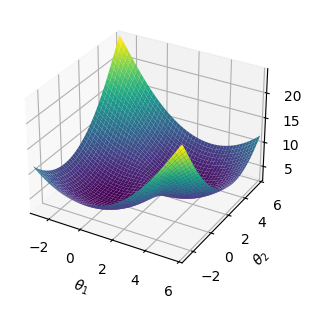
\includegraphics[scale=0.8, max width=\linewidth]{./fig/bayesian-brain/mcmc/cell004.png}
	\caption{cell004.png}
	\label{cell004.png}
\end{figure}
Metropolis-Hastings法における採用・不採用アルゴリズム.
\begin{lstlisting}[language=julia]
# Metropolis-Hastings method; log_p: unnormalized log-posterior
function gaussian_mh(log_p::Function, θ_init::Vector{Float64}, σ::Float64, num_iter::Int)
    d = length(θ_init)
    samples = zeros(d, num_iter)
    num_accepted = 0
    θ = θ_init # init position
    for m in 1:num_iter
        θ_ = rand(MvNormal(θ, σ*I))
        mH = log_p(θ) + logpdf(MvNormal(θ, σ*I), θ_)       # initial Hamiltonian
        mH_ = log_p(θ_) + logpdf(MvNormal(θ_, σ*I), θ)    # final Hamiltonian
        
        if min(1, exp(mH_ - mH)) > rand()
            θ = θ_ # accept
            num_accepted += 1
        end
        samples[:, m] = θ
    end
    return samples, num_accepted
end;
\end{lstlisting}
\begin{lstlisting}[language=julia]
log_p(θ) = logpdf(mixed_gauss, θ);
grad(θ)= ForwardDiff.gradient(log_p, θ)
\end{lstlisting}
\begin{lstlisting}[language=julia]
θm, num_accepted = gaussian_mh(log_p, [1.0,0.5], 1.0, 2000)
\end{lstlisting}
\begin{lstlisting}[language=julia]
size(θm)
\end{lstlisting}
\begin{lstlisting}[language=julia]
Um = kde((θm[1, :], θm[2, :]));

fig, ax = subplots(1, 2, figsize=(5, 3), sharex="all", sharey="all")
fig.suptitle("Metropolis-Hastings method")
ax[1].set_title("Raw trace")
ax[1].contour(x, x, -mixed_gauss_heat)
ax[1].plot(θm[1, :], θm[2, :], color="tab:red", alpha=0.5)
ax[1].set_xlim(-3,6); ax[1].set_ylim(-3,6)
ax[2].set_title("Density")
ax[2].contourf(Um.x, Um.x, Um.density)
fig.tight_layout()
\end{lstlisting}
\begin{figure}[ht]
	\centering
	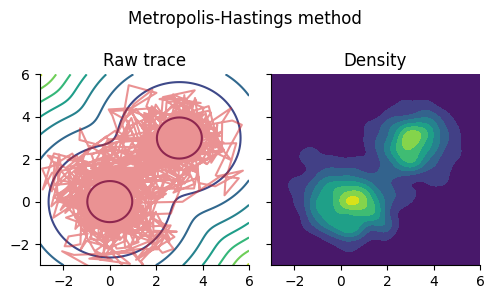
\includegraphics[scale=0.8, max width=\linewidth]{./fig/bayesian-brain/mcmc/cell010.png}
	\caption{cell010.png}
	\label{cell010.png}
\end{figure}
\subsection{ランジュバン・モンテカルロ法 (LMC)}
拡散過程
\begin{equation}
{\frac{d\theta}{dt}}=\nabla \log p (\theta)+{\sqrt 2}{d{W}}
\end{equation}
Euler–Maruyama法により,
\begin{lstlisting}[language=julia]
nt = 10000
ϵ = 0.1
\end{lstlisting}
\begin{lstlisting}[language=julia]
β = 1
ρ = sqrt(2*ϵ);
\end{lstlisting}
\begin{lstlisting}[language=julia]
θl = zeros(nt, 2)
θ = [1.0,0.5]
for t in 1:nt
    θ += ϵ * β * grad(θ) + ρ * randn(2)
    θl[t, :] = θ
end
\end{lstlisting}
\begin{lstlisting}[language=julia]
Ul = kde((θl[:, 1], θl[:, 2]));

fig, ax = subplots(1, 2, figsize=(5, 3), sharex="all", sharey="all")
fig.suptitle("Langevin dynamics")
ax[1].set_title("Raw trace")
ax[1].contour(x, x, -mixed_gauss_heat)
ax[1].plot(θl[:, 1], θl[:, 2], color="tab:red", alpha=0.5)
ax[1].set_xlim(-3,6); ax[1].set_ylim(-3,6)
ax[2].set_title("Density")
ax[2].contourf(Ul.x, Ul.x, Ul.density)
fig.tight_layout()
\end{lstlisting}
\begin{figure}[ht]
	\centering
	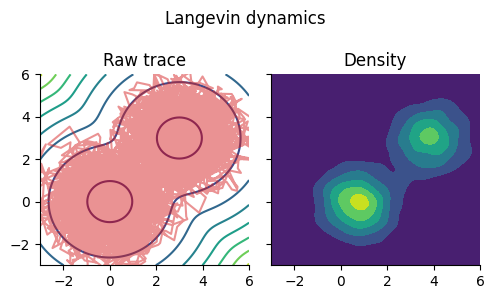
\includegraphics[scale=0.8, max width=\linewidth]{./fig/bayesian-brain/mcmc/cell015.png}
	\caption{cell015.png}
	\label{cell015.png}
\end{figure}
\subsection{ハミルトニアン・モンテカルロ法 (HMC法)}
LMCよりも一般的なMCMCの手法としてHamiltonianモンテカルロ法(Hamiltonian Monte Calro; HMC)あるいはハイブリッド・モンテカルロ法(Hybrid Monte Calro)がある.エネルギーポテンシャルの局面上をHamilton力学に従ってパラメータを運動させることにより高速にサンプリングする手法である.
一般化座標を$\mathbf{q}$, 一般化運動量を$\mathbf{p}$とする.ポテンシャルエネルギーを$U(\mathbf{q})$としたとき,古典力学 (解析力学) において保存力のみが作用する場合の\textbf{ハミルトニアン (Hamiltonian)}\index{はみるとにあん (Hamiltonian)@ハミルトニアン (Hamiltonian)} $\mathcal{H}(\mathbf{q}, \mathbf{p})$は
\begin{equation}
\mathcal{H}(\mathbf{q}, \mathbf{p})\triangleqU(\mathbf{q})+\frac{1}{2}\|\mathbf{p}\|^2
\end{equation}
となる.このとき,次の2つの方程式が成り立つ.
\begin{equation}
\frac{d\mathbf{q}}{dt}=\frac{\partial \mathcal{H}}{\partial \mathbf{p}}=\mathbf{p},\quad\frac{d\mathbf{p}}{dt}=-\frac{\partial \mathcal{H}}{\partial \mathbf{q}}=-\frac{\partial U}{\partial \mathbf{q}}
\end{equation}
これを\textbf{ハミルトンの運動方程式(hamilton's equations of motion)}\index{はみるとんのうんどうほうていしき(hamilton's equations of motion)@ハミルトンの運動方程式(hamilton's equations of motion)} あるいは\textbf{正準方程式 (canonical equations)}\index{せいじゅんほうていしき (canonical equations)@正準方程式 (canonical equations)} という.
リープフロッグ(leap frog)法により離散化する.
\begin{lstlisting}[language=julia]
function leapfrog(grad::Function, θ::Vector{Float64}, p::Vector{Float64}, ϵ::Float64, L::Int)
    for l in 1:L
        p += 0.5 * ϵ * grad(θ)
        θ += ϵ * p
        p += 0.5 * ϵ * grad(θ)
    end
    return θ, p
end;
\end{lstlisting}
\begin{lstlisting}[language=julia]
# Hamiltonian Monte Carlo method; log_p: unnormalized log-posterior
function hmc(log_p::Function, θ_init::Vector{Float64}, ϵ::Float64, L::Int, num_iter::Int)
    grad(θ)= ForwardDiff.gradient(log_p, θ)
    d = length(θ_init)
    samples = zeros(d, num_iter)
    num_accepted = 0
    θ = θ_init # init position
    for m in 1:num_iter
        p = randn(d) # get momentum        
        H = -log_p(θ) + 0.5 * p' * p        # initial Hamiltonian
        θ_, p_ = leapfrog(grad, θ, p, ϵ, L) # update
        H_ = -log_p(θ_) + 0.5 * p_' * p_    # final Hamiltonian
        
        if min(1, exp(H - H_)) > rand()
            θ = θ_ # accept
            num_accepted += 1
        end
        samples[:, m] = θ
    end
    return samples, num_accepted
end;
\end{lstlisting}
\begin{lstlisting}[language=julia]
ps = zeros(nt, 2)
θs = zeros(nt, 2)
p = randn(2)
θ = randn(2)
for t in 1:nt
    if t in 20:10:nt
        p = randn(2)
    end
    p += 0.5 * ϵ * grad(θ)
    θ += ϵ * p
    p += 0.5 * ϵ * grad(θ)
    ps[t, :] = p
    θs[t, :] = θ
end
\end{lstlisting}
\begin{lstlisting}[language=julia]
Us = kde((θs[:, 1], θs[:, 2]));
\end{lstlisting}
\begin{lstlisting}[language=julia]
fig, ax = subplots(1, 2, figsize=(5, 3), sharex="all", sharey="all")
fig.suptitle("Hamiltonian dynamics")
ax[1].set_title("Raw trace")
ax[1].contour(x, x, -mixed_gauss_heat)
ax[1].plot(θs[:, 1], θs[:, 2], color="tab:red", alpha=0.5)
ax[1].set_xlim(-3,6); ax[1].set_ylim(-3,6)
ax[2].set_title("Density")
ax[2].contourf(Us.x, Us.x, Us.density)
fig.tight_layout()
\end{lstlisting}
\begin{figure}[ht]
	\centering
	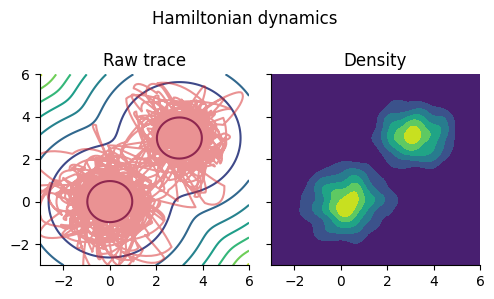
\includegraphics[scale=0.8, max width=\linewidth]{./fig/bayesian-brain/mcmc/cell021.png}
	\caption{cell021.png}
	\label{cell021.png}
\end{figure}
*ToDo: 自己相関確認する*
\subsection{線形回帰への適応}
\begin{lstlisting}[language=julia]
# Generate Toy datas
num_train, num_test = 20, 100 # sample size
dims = 4 # dimensions
σy = 0.3

polynomial_expansion(x; degree=3) = stack([x .^ p for p in 0:degree]);

Random.seed!(0);
x = rand(num_train)
y = sin.(2π*x) + σy * randn(num_train);
ϕ = polynomial_expansion(x, degree=dims-1) # design matrix

xtest = range(-0.1, 1.1, length=num_test)
ytest = sin.(2π*xtest)
ϕtest = polynomial_expansion(xtest, degree=dims-1);
\end{lstlisting}
\begin{lstlisting}[language=julia]
log_joint(w, ϕ, y, σy, μ₀, Σ₀) = sum(logpdf.(Normal.(ϕ * w, σy), y)) + logpdf(MvNormal(μ₀, Σ₀), w);
\end{lstlisting}
\begin{lstlisting}[language=julia]
α, β = 5e-3, 5.0
\end{lstlisting}
\begin{lstlisting}[language=julia]
w = randn(dims)
μ₀ = zeros(dims)
Σ₀ = 1/α * I;
\end{lstlisting}
\begin{lstlisting}[language=julia]
ulp(w) = log_joint(w, ϕ, y, σy, μ₀, Σ₀)
\end{lstlisting}
\begin{lstlisting}[language=julia]
w_init = rand(MvNormal(μ₀, Σ₀), 1)[:, 1]
\end{lstlisting}
\begin{lstlisting}[language=julia]
@time samples, num_accepted = hmc(ulp, w_init, 1e-2, 10, 500)
\end{lstlisting}
\begin{lstlisting}[language=julia]
plot(samples[1, :])
\end{lstlisting}
\begin{figure}[ht]
	\centering
	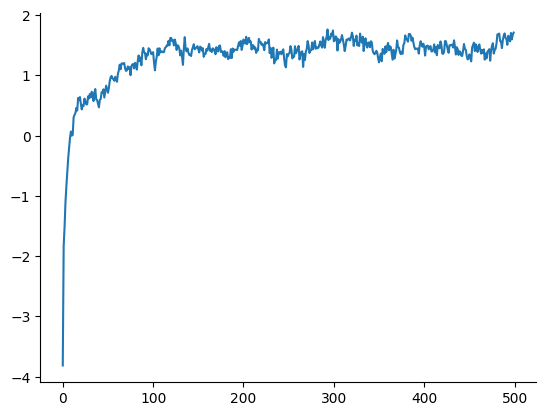
\includegraphics[scale=0.8, max width=\linewidth]{./fig/bayesian-brain/mcmc/cell031.png}
	\caption{cell031.png}
	\label{cell031.png}
\end{figure}
\begin{lstlisting}[language=julia]
yhmc = ϕtest * samples[:, 300:end];
yhmc_mean = mean(yhmc, dims=2)[:];
yhmc_std = std(yhmc, dims=2)[:];
\end{lstlisting}
\begin{lstlisting}[language=julia]
figure(figsize=(5,3.5))
title("Bayesian Linear Regression")
scatter(x, y, facecolor="None", edgecolors="black", s=25) # samples
plot(xtest, ytest, "--", label="Actual", color="tab:red")  # regression line
plot(xtest, yhmc_mean, label="Predicted mean", color="tab:blue")  # regression line
fill_between(xtest, yhmc_mean+yhmc_std, yhmc_mean-yhmc_std, alpha=0.5, color="tab:gray", label="Predicted std.")
for i in 1:5
    plot(xtest, yhmc[:, end-i], alpha=0.3, color="tab:green")
end
xlabel("x"); ylabel("y"); legend()
xlim(-0.1, 1.1); tight_layout()
\end{lstlisting}
\begin{figure}[ht]
	\centering
	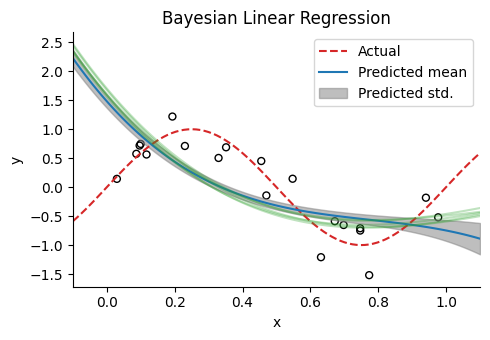
\includegraphics[scale=0.8, max width=\linewidth]{./fig/bayesian-brain/mcmc/cell033.png}
	\caption{cell033.png}
	\label{cell033.png}
\end{figure}
